\documentclass[9pt,aspectratio=169]{beamer}

\usepackage{nicefrac}
\usepackage{tabularx}
\newcolumntype{Y}{>{\centering\arraybackslash\leavevmode}X}
\renewcommand\tabularxcolumn[1]{m{#1}}% for vertical centering text in X column
\usepackage{luamplib}
\everymplib{input mpcolornames; input repere; input macros;beginfig(1);}
\everyendmplib{endfig;}

\usetheme{graham}

\title{Right Triangles}
\subtitle[Graham Middle School]{Graham Middle School Math Olympiad Team}

\begin{document}
\maketitle

\begin{frame}{Right triangles and the Pythagorean theorem}
  \begin{columns}[T]
    \begin{column}{0.5\textwidth}
      A triangle with a $90°$ angle is called a \textbf{right triangle}.  The two sides that meet to form the right angle are called the \textbf{legs} of the triangle.  The long side opposite the right angle is called the \textbf{hypotenuse}. 

      \begin{definition}
        \textbf{Pythagorean Theorem:}
        
        If the legs of a right triangle have lengths $a$ and $b$, and the hypotenuse has length $c$, then 
        \[ a^2 + b^2 = c^2.\]
        \vspace*{-\baselineskip}
      \end{definition}
      This theorem is today named after the 6th century B.C. Greek/Ionian philosopher Pythagoras, but it was known in China and India prior to his birth.  There are literally hundreds of proofs of this theorem, and one example is given on this page.
      \begin{center}
        \leavevmode
        \begin{mplibcode}
          u = 1cm;
          repere(-5,5,u,-5,5,u);
            pair A, B, C;
            A := (0, 0);
            B := (3, 0);
            C := (0, 1.3);
            draw A--B--C--cycle withpen pencircle scaled 1.25;
            draw marqueangledroit(B,A,C);
            label.lft(btex $a$ etex, 0.5[A, C]);
            label.bot(btex $b$ etex, 0.5[A, B]);
            label.urt(btex $c$ etex, 0.45[C, B]);
            label.rt(btex $a^2 + b^2 = c^2$ etex, (2.5, 1));
          fin;
        \end{mplibcode}
      \end{center}

    \end{column}
    \begin{column}{0.5\textwidth}
      The earliest version of the proof we’re showing here comes from China.  Arrange four identical right triangles as shown in the diagram.\smallskip

      \begin{tabularx}{\textwidth}{YY}
        \begin{mplibcode}
          u = 0.9cm;
          repere(-5,5,u,-1,5,u);
            fill (1, 0)--(3, 1)--(2, 3)--(0, 2)--cycle withcolor lime;
            draw (0, 0)--(3, 0)--(3, 3)--(0, 3)--cycle withpen pencircle scaled 1.25;
            draw (1, 0)--(3, 1)--(2, 3)--(0, 2)--cycle withpen pencircle scaled 1.25;
            label.lft(btex $a$ etex, (0, 2.5));
            label.lft(btex $b$ etex, (0, 1));
            label.top(btex $a$ etex, (2.5, 3));
            label.top(btex $b$ etex, (1, 3));
            picture c[];
            c1 := thelabel.lrt(btex $c$ etex, 0.55[(2, 3),(0, 2)]);
            c2 := thelabel.urt(btex $c$ etex, 0.45[(1, 0),(0, 2)]);
            unfill bbox c1;
            draw c1;
            unfill bbox c2;
            draw c2;
            c3 := thelabel(btex $c^2$ etex, (1.5, 1.5));
            unfill bbox c3;
            draw c3;
          fin;
        \end{mplibcode}
        &
        \begin{mplibcode}
          u = 0.9cm;
          repere(-5,5,u,-1,5,u);
            fill (0, 0)--(2, 0)--(2, 2)--(0, 2)--cycle withcolor rose;
            fill (2, 2)--(3, 2)--(3, 3)--(2, 3)--cycle withcolor cyan;
            draw (0, 0)--(3, 0)--(3, 3)--(0, 3)--cycle withpen pencircle scaled 1.25;
            draw (0, 2)--(3, 2) withpen pencircle scaled 1.25;
            draw (2, 0)--(2, 3) withpen pencircle scaled 1.25;
            draw (0, 2)--(2, 3) withpen pencircle scaled 1.25;
            draw (2, 2)--(3, 0) withpen pencircle scaled 1.25;
            label.lft(btex $a$ etex, (0, 2.5));
            label.lft(btex $b$ etex, (0, 1));
            label.top(btex $a$ etex, (2.5, 3));
            label.top(btex $b$ etex, (1, 3));
            picture c[];
            c1 := thelabel(btex $a^2$ etex, (2.5, 2.5));
            c2 := thelabel(btex $b^2$ etex, (1, 1));
            unfill bbox c1;
            draw c1;
            unfill bbox c2;
            draw c2;
          fin;
        \end{mplibcode}
      \end{tabularx}\smallskip

      We create an outer square with sides $a+b$ and an inner square whose sides are the length of the hypotenuse, $c$. The total area of the outer square is $(a+b)^2 = a^2 + 2ab + b^2$.  This has to equal the area of the four triangles: $4 \frac{ab}{2}$ plus the area of the central square: $c^2$.
      
      So $a^2 + 2ab + b^2  = 2ab + c^2$.  Canceling the $2ab$ on both sides we prove:  $a^2 + b^2 = c^2$.
    \end{column}
  \end{columns}
\end{frame}

\begin{frame}{Pythagorean triples}
  \begin{columns}[T]
    \begin{column}{0.5\textwidth}
      The Pythagorean Theorem often leads to answers with square roots in them (we’ll see some important examples later in this lesson).  Math contests, though, typically like clean answers that emphasize your grasp of the math and don’t get bogged down with calculations.  That is why Pythagorean Triples show up in math contests so often.  
      
      \textbf{Pythagorean triples} are sets of $3$ integers that satisfy the Pythagorean condition that the sum of the squares of two integers equals the square of the third integer.  One such triple is $3$, $4$, $5$ since $9 + 16 = 25$.  It will be helpful in contests to memorize the most commonly seen Pythagorean Triples.

      \begin{definition}
        Most Common Pythagorean Triples
        \[ (3,\ 4,\ 5)\ \ (5,\ 12,\ 13)\ \ (8,\ 15,\ 17)\ \ (7,\ 24,\ 25)\]
        \vspace*{-\baselineskip}
      \end{definition}
    \end{column}
    \begin{column}{0.5\textwidth}
      \begin{problem}
        If we multiply all of the elements in a Pythagorean Triple by the same constant, the resulting triplet still satisfies the Pythagorean relation. 
      \end{problem}
      This is easily shown using the distributive property.  Suppose $a^2 + b^2 = c^2$
      
      What happens when we multiply each element by $a$ constant $n$?  Does $(na)^2 + (nb)^2 = (nc)^2$ ?  Factoring out the common $n^2$, $n^2 (a^2 + b^2) = n^2 c^2$  Then canceling the $n^2$ from both sides of the equation shows that the relation is still true.\smallskip

      For example, since $3$, $4$, $5$ is a Pythagorean triple, so too is $6$, $8$, $10$.  Of course, the constant we multiply by can also be a fraction.  Multiplying each element by $\nicefrac{1}{4}$, we see that $\nicefrac{3}{4}$, $1$, $\nicefrac{5}{4}$ satisfies the Pythagorean relationship as well.

      \begin{example}
        All Pythagorean Triplets may be obtained by taking any counting numbers $m > n$:
        \[ a = m^2 - n^2,\quad b = 2mn, \quad c = m^2 + n^2. \]
        \vspace*{-\baselineskip}
      \end{example}
    \end{column}
  \end{columns}
\end{frame}

\begin{frame}{Converse Pythagorean theorem}
  \begin{columns}[T]
    \begin{column}{0.5\textwidth}
      \begin{definition}
        If the square of the largest length in a triangle is equal to the sum of the squares of the two smaller sides, then that triangle \textbf{must} be a right triangle.
      \end{definition}
      To prove this, construct right triangle $ABC$ and another triangle $DEF$  such that leg lengths $AB$ and $BC$ are equal to $DE$ and $EF$.  Since we are given the sum of the squares of the two smaller sides is equal to the square of the largest length, then the largest length of triangle $DEF$, $DF$ must be equal to the hypotenuse $AC$.  
      
      By \textbf{SSS} similarity, $ABC$ is similar to $DEF$, so $\angle ABC$ is congruent to $\angle DEF$ and $DEF$ is a right triangle.\smallskip

      \begin{tabularx}{\textwidth}{YY}
        \begin{mplibcode}
          u = 0.9cm;
          taille_marque_s := 0.15cm;
          angle_marque_s := 90;
          repere(-5,5,u,-1,5,u);
            pair A, B, C;
            A := (0, 0);
            B := (3, 0);
            C := (0, 1.3);
            draw A--B--C--cycle withpen pencircle scaled 1.25;
            draw marqueangledroit(B,A,C);
            label.ulft(btex $A$ etex, C);
            label.llft(btex $B$ etex, A);
            label.bot(btex $C$ etex, B);
            draw marquesegment(A,C,1);
            draw marquesegment(A,B,2);
          fin;
        \end{mplibcode}
        &
        \begin{mplibcode}
          u = 0.9cm;
          taille_marque_s := 0.15cm;
          angle_marque_s := 90;
          repere(-5,5,u,-1,5,u);
            pair A, B, C;
            A := (0, 0);
            B := (3, 0);
            C := (0, 1.3);
            draw A--B--C--cycle withpen pencircle scaled 1.25;
            label.urt(btex $?$ etex, A shifted (0.1, 0.1));
            label.ulft(btex $D$ etex, C);
            label.llft(btex $E$ etex, A);
            label.bot(btex $F$ etex, B);
            draw marquesegment(A,C,1);
            draw marquesegment(A,B,2);
          fin;
        \end{mplibcode}
      \end{tabularx}
    \end{column}
    \begin{column}{0.5\textwidth}
      The relationship between the square of the length of the longest side and the sum of the squares of the lengths of the shorter sides can tell us if a triangle is acute or obtuse.
      
      \begin{tabularx}{\textwidth}{YY}
        \begin{mplibcode}
          u = 0.9cm;
          taille_marque_s := 0.15cm;
          angle_marque_s := 90;
          repere(-5,5,u,-1,5,u);
            pair A, B, C;
            A := (0, 0);
            B := (2, 0);
            C := (-1, 2.5);
            draw A--B--C--cycle withpen pencircle scaled 1.25;
            label.lft(btex $b$ etex, 0.5[A, C]);
            label.bot(btex $a$ etex, 0.5[A, B]);
            label.urt(btex $c$ etex, 0.5[B, C]);
            label.urt(btex $\theta$ etex, A shifted (-0.05, 0));
          fin;
        \end{mplibcode}
        & 
        \begin{mplibcode}
          u = 0.9cm;
          taille_marque_s := 0.15cm;
          angle_marque_s := 90;
          repere(-5,5,u,-1,5,u);
            pair A, B, C;
            A := (0, 0);
            B := (2, 0);
            C := (0.5, 2.5);
            draw A--B--C--cycle withpen pencircle scaled 1.25;
            label.lft(btex $b$ etex, 0.5[A, C]);
            label.bot(btex $a$ etex, 0.5[A, B]);
            label.urt(btex $c$ etex, 0.5[B, C]);
            label.urt(btex $\theta$ etex, A shifted (0.05, 0));
          fin;
        \end{mplibcode} \\
        \begin{minipage}{0.45\columnwidth}
          \begin{example}
            If $a^2 + b^2 < c^2$, then the triangle is obtuse.
          \end{example}           
        \end{minipage}
        & 
        \begin{minipage}{0.45\columnwidth}
          \begin{example}
            If $a^2 + b^2 > c^2$, then the triangle is acute.
          \end{example}
        \end{minipage}
      \end{tabularx}\smallskip

      Finally we note that as $\theta$ approaches $180°$, length $c$ approaches the sum $a + b$, while when $θ$ approaches $0°$, length $c$ approaches zero.
    \end{column}
  \end{columns}
\end{frame}

\begin{frame}{45-45-90 triangles}
  \begin{columns}[T]
    \begin{column}{0.5\textwidth}
      Let’s consider an isosceles right triangle like the one shown below.  In an isosceles triangle, the base angles are congruent, and (since the sum of the angles is $180°$) measure $45°$.  Such a triangle is often referred to as a $45\mbox{--}45\mbox{--}90$ triangle.  Using the Pythagorean Theorem, $a^2 + b^2 = c^2$  but $b^2 = a^2$ so $2a^2 = c^2$. Taking the square root of both sides, $c = \sqrt{2} a$

      \begin{center}
        \leavevmode
        \begin{mplibcode}
          u = 1cm;
          repere(-5,5,u,-5,5,u);
            pair A, B, C;
            A := (0, 0);
            B := (3, 0);
            C := (0, 3);
            draw A--B--C--cycle withpen pencircle scaled 1.25;
            draw marqueangledroit(B,A,C);
            label.lft(btex $a$ etex, 0.5[A, C]);
            label.bot(btex $a$ etex, 0.5[A, B]);
            label.urt(btex $\sqrt{2} a$ etex, 0.45[C, B]);
            taille_marque_a := 0.5cm;
            draw marqueangle(C, B, A, 1);
            nomme(C, B, A, btex $45°$ etex);
            draw marqueangle(A, C, B, 1);
            taille_marque_a := 0.6cm;
            nomme(A, C, B, btex $45°$ etex);
          fin;
        \end{mplibcode}
      \end{center}

    \end{column}
    \begin{column}{0.5\textwidth}
      \begin{definition}
        The diagonal of a square divides it into two congruent $45\mbox{--}45\mbox{--}90$ triangles. 
      \end{definition}\medskip

      \begin{tabularx}{\textwidth}{YX}
        \begin{mplibcode}
          u = 0.9cm;
          repere(-5,5,u,-1,5,u);
            draw (0, 0)--(0, 3)--(3, 3)--(3, 0)--cycle withpen pencircle scaled 1.25;
            draw (0, 3)--(3, 0);
            label.lft(btex $a$ etex, (0, 1.5)); 
            label.bot(btex $a$ etex, (1.5, 0)); 
            label.urt(btex $\sqrt{2} a$ etex, (1.45, 1.45));
          fin;
        \end{mplibcode}
        & 
        The area of the square, $a^2$, is equal to $\nicefrac{1}{2}$ times the square of its diagonal.\\[0.5ex]
        \begin{mplibcode}
          u = 0.9cm;
          repere(-5,5,u,-1,5,u);
            draw (0, 0)--(0, 3)--(3, 3)--(3, 0)--cycle withpen pencircle scaled 1.25;
            draw (0, 3)--(3, 0);
            draw (0, 0)--(3, 3);
            draw marqueangledroit((3, 3), (1.5, 1.5), (0, 3));
            label.lft(btex $a$ etex, (0, 1.5)); 
            label.bot(btex $a$ etex, (1.5, 0)); 
            label.ulft(btex $\frac{\sqrt{2} a}{2}$ etex, (0.9, 0.6));
            label.urt(btex $\frac{\sqrt{2} a}{2}$ etex, (2.1, 0.6));
          fin;
        \end{mplibcode}
        & 
        Intersecting diagonals divide a square into four equal $45\mbox{--}45\mbox{--}90$ triangles, with hypotenuse $a$, and legs~$\dfrac{\sqrt{2}a}{2}$.
      \end{tabularx}
    \end{column}
  \end{columns}
\end{frame}

\begin{frame}{30-60-90 triangles}
  \begin{columns}[T]
    \begin{column}{0.5\textwidth}
      Suppose you have an equilateral triangle of side length $s$.  What is its area?
      
      To calculate this, we need to know the length of an altitude, so let’s draw a line from the top vertex that is perpendicular to the base of the triangle.  By symmetry, that altitude \textbf{bisects} (splits into two equal halves) the vertex angle and the base, so we create a pair of congruent right triangles with angles $30\mbox{--}60\mbox{--}90$.\medskip

      \begin{tabularx}{\textwidth}{YX}
        \begin{mplibcode}
          u = 1.1cm;
          repere(-5,5,u,-1,5,u);
            pair A, B, C, D;
            A := (0, 0);
            B := (3, 0);
            C := (1.5, 2.6);
            D := 0.5[A, B];
            draw A--B--C--cycle withpen pencircle scaled 1.25;
            draw D--C;
            label.ulft(btex $s$ etex, 0.5[A, C]); 
            label.urt(btex $s$ etex, 0.5[B, C]); 
            label.bot(btex $\nicefrac{s}{2}$ etex, 0.5[A, D]); 
            label.bot(btex $\nicefrac{s}{2}$ etex, 0.5[B, D]); 
            label.lft(btex $h$ etex, 0.4[D, C]);
            taille_marque_a := 0.8cm;
            nomme(A, C, D, btex $30°$ etex);
            nomme(D, C, B, btex $30°$ etex);
            taille_marque_a := 0.7cm;
            draw marqueangle(A, C, D, 1);
            draw marqueangle(D, C, B, 1);
            taille_marque_a := 0.4cm;
            nomme(C, B, D, btex $60°$ etex);
            nomme(B, A, C, btex $60°$ etex);
            draw marqueangle(C, B, D, 2);
            draw marqueangle(B, A, C, 2);
            draw marqueangledroit(B, D, C);
          fin;
        \end{mplibcode}
        & 
        Using the Pytha\-go\-rean Theorem, 
        {\begin{align*}
          \left(\frac{s}{2}\right)^2 + h^2 &= s^2 \\
          h^2 &= \frac{3}{4} s^2 \\
          h &= \frac{\sqrt{3}s}{2}.
        \end{align*}}
      \end{tabularx}
    \end{column}
    \begin{column}{0.5\textwidth}
      \begin{definition}
        The area of an equilateral triangle of side length $s$ is $\dfrac{\sqrt{3} s^2}{4}$.
      \end{definition}
      
      \begin{definition}
        In a $30\mbox{--}60\mbox{--}90$ triangle with hypotenuse length $s$, the side opposite the $30°$ angle has length $\dfrac{s}{2}$, while the side opposite the $60°$ angle has length $\dfrac{\sqrt{3}s}{2}$.
      \end{definition}

      Rather than trying to memorize these relationships, I find it useful to recall how we came up with them using the Pythagorean theorem, and re-derive the formulae when needed.  It is handy, however, to recall that the side opposite the $30°$ angle is half the length of the hypotenuse.
    \end{column}
  \end{columns}
\end{frame}

\begin{frame}{Right angles in the cartesian plane}
  \begin{columns}[T]
    \begin{column}{0.5\textwidth}
      \begin{definition}
        \textbf{Theorem:}
        
        If two lines intersect at a \textbf{right angle} in a coordinate plane, then \textbf{the product of their slopes is~$-1$}, unless the lines are parallel to the $x$- and $y$-axes.  In other words, the product of the slopes of perpendicular lines is $-1$.
      \end{definition}

      \begin{wrapfigure}{l}{0.4\textwidth}
        \vspace*{-1em}
        \begin{mplibcode}
          u = 1cm;
          repere(-1.3,2,u,-1.7,1.3,u);
            draw axes(0,0);
            pair A, B, O;
            O := origin;
            A := (1, 0.8);
            B := (1, -1/0.8);
            draw O--A withcolor bleu withpen pencircle scaled 1.25;
            draw O--B withcolor rouge withpen pencircle scaled 1.25;
            draw B--A withcolor vertfonce withpen pencircle scaled 1.25;
            nomme.top(O, btex $$ etex);
            nomme.top(A, btex $(1,\ m_1)$ etex);
            nomme.bot(B, btex $(1,\ m_2)$ etex);
          fin;
        \end{mplibcode}
        \vspace*{-1em}
      \end{wrapfigure}

      Proof: 
      
      In the diagram, let two lines with slopes $m_1$ and $m_2$ intersect at the origin.  By the converse Pythagorean theorem, if the sum of the squares of the lengths of the blue and red lines, equals the square of the length of the green line, then they must be perpendicular.

      Square of the length of the blue line $= 1 + m_1^2$.
      
      Square of the length of red line $= 1 + m_2^2$.
    \end{column}
    \begin{column}{0.5\textwidth}
      Square of the length of green line $=$ $= (m_1-m_2)^2 = m_1^2 + m_2^2 - 2 m_1 m_2$.
      \[ (\text{blue length})^2 + (\text{red length})^2 = 2 + m_1^2 + m_2^2. \]
      When $(\text{blue length})^2 + (\text{red length})^2 = (\text{green length})^2$, we must have a $90°$ angle.  This occurs when $2 + m_1^2 + m_2^2 = m_1^2 + m_2^2 - 2 m_1 m_2$ which simplifies to:
      \[ 2 = – 2 m_1 m_2 \quad \text{or}\quad m_1 m_2 = -1.\]\vspace*{-1.3\baselineskip}
      \begin{flushright}Q.E.D.\end{flushright}
      \begin{problem}
        If line $AO$ with slope $-\nicefrac{1}{2}$ intersects at the origin, point $O$, with line $OB$ perpendicular to line $AO$, what is the $y$-coordinate of point $B$, if its $x$-coordinate is~$5$?
      \end{problem}
      If $OB$ is perpendicular to $AO$, the slope of $OB$ must be $2$.  Since $OB$ passes through the origin with slope $2$, point $B$ must be at $(5,\ 10)$.
    \end{column}
  \end{columns}
\end{frame}

\begin{frame}{Geometric mean}
  \begin{columns}[T]
    \begin{column}{0.5\textwidth}
      \begin{definition}
        \textbf{Theorem}

        In a triangle with a right angle at vertex $A$, the altitude drawn from $A$ to the opposite side divides that side into two segments such that the product of the length of those two segments is equal to the length of the altitude squared. 
      \end{definition}

      \begin{wrapfigure}{l}{0.4\textwidth}
        \begin{mplibcode}
          u = 0.8cm;
          repere(-5,5,u,-5,6,u);
            pair A, B, C, D;
            A := (0, 0);
            B := (3, 0);
            C := (0, 4.5);
            D - A = whatever*((B - C) rotated 90);
            D = whatever[B, C];
            draw A--B--C--cycle withpen pencircle scaled 1.25;
            draw A--D withpen pencircle scaled 1.25;
            draw marqueangledroit(B,A,C);
            draw marqueangledroit(B,D,A);
            nomme.llft(A, btex $A$ etex);
            nomme.lrt(B, btex $B$ etex);
            nomme.top(C, btex $C$ etex);
            nomme.urt(D, btex $D$ etex);
            draw marqueangle(C, B, A, 2);
            taille_marque_a := 0.5cm;
            draw marqueangle(A, C, B, 1);
            draw marqueangle(B, A, D, 1);
            draw marqueangle(D, A, C, 2);
          fin;
        \end{mplibcode}
        \vspace*{-1em}
      \end{wrapfigure}
      
      Proof:

      $\triangle CAB$ is similar to $\triangle CDA$ by \textbf{AA}.

      $\triangle CAB$ is similar to $\triangle ADB$ by \textbf{AA}.

      $\triangle CDA$ is similar to $\triangle ADB$ by the transitive property of similarity. From the proportionality of side lengths in similar triangles, we have $CD/AD$ = $AD/DB$ so
      $ (CD)(DB) = (AD)^2.$
      
    \end{column}
    \begin{column}{0.5\textwidth}
      We could also express this relationship as
      \[ AC = \sqrt{(CD) (DB)}. \]
      The square root of the product of two numbers is known as the \textbf{geometric mean}.  It can be generalized to taking the $n$\textsuperscript{th} root of the product of $n$ terms.   It is a different way of averaging terms than the arithmetic mean.  The reason this method of averaging is known as a geometric mean is due to its frequent appearance in geometric relationships such as the one in this example.
    \end{column}
  \end{columns}
\end{frame}

\begin{frame}{Aria of a triangle}
  \begin{columns}[T]
    \begin{column}{0.5\textwidth}
      \begin{definition}
        For a triangle with base $b$ and height $h$, the area $A$ is given by $A = \dfrac{bh}{2}$.
      \end{definition}
      \begin{wrapfigure}[8]{l}{20.00mm}
        \begin{mplibcode}
          u := 1cm;
          fill (0u, 0u)--(1u, 2u)--(3u, 0u)--cycle withcolor 0.7white;
          Draw (0u, 0u)--(3u, 0u)--(3u, 2u)--(0u, 2u)--cycle, (0u, 0u)--(1u, 2u)--(3u, 0u), (1u, 0u)--(1u, 2u);
          label.bot(btex $b$ etex, (1.5u, 0u));
          label.rt(btex $h$ etex, (1u, 1u));
        \end{mplibcode}
      \end{wrapfigure}
      Observe that this is exactly half the area of a rectangle which has the same base and height. A logical reasoning for this is that you can make two triangles by dropping an altitude for which both halves are each rotated $180$ degrees about their hypotenuse's mid-point to form two rectangles. Thus it is clear that the triangles are one half the area of their respective rectangles which have a total area of $bh$.
    \end{column}
    \begin{column}{0.5\textwidth}
      \vspace*{-2\baselineskip}
      Knowing sides of triangle allows us to calculate area using the \emph{Heron's formula}.
      \begin{definition}
        \textbf{Heron's formula} states that the area is 
        \[A = \sqrt{p(p-a)(p-b)(p-c)},\] 
        where $a$, $b$, $c$ are the lengths of sides, and $p$ is the triangle's semi-perimeter $\dfrac{a+b+c}{2}$.
      \end{definition}

      And we also calculate area of triangle knowing coordinates of points using the \emph{Shoelace formula}
      \begin{definition}
        \textbf{Shoelace formula} 
        \[A = \frac{x_1 y_2 + x_2 y_3 + x_3 y_1 - x_1 y_3 - x_2 y_1 - x_3 y_2}{2}. \] Where $(x_1,\ y_1)$, $(x_2,\ y_2)$, and $(x_3,\ y_3)$ are coordinates of vertices of a triangle.
      \end{definition}
      \begin{wrapfigure}{l}{25.00mm}
        \vspace*{-\intextsep}
        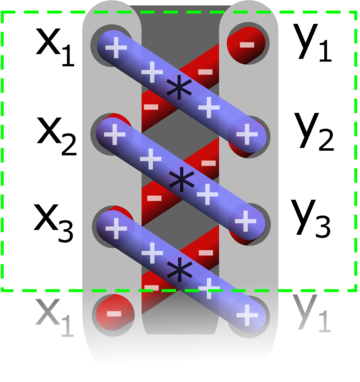
\includegraphics[width=2.5cm]{12 - Right Triangles/Shoelace3.png}
        \vspace*{-\intextsep}
      \end{wrapfigure}
      The picture on the left show the way to remember this formula. The generalization of this formula allows to calculate area of a polygon with may sides.
    \end{column}
  \end{columns}
\end{frame}

% \begin{frame}{Exercises}
%   \begin{columns}[T]
%     \begin{column}{0.5\textwidth}
%       \setlength{\leftmargini}{0.2cm}
%       \begin{enumerate}
%         \item The figure below is used for exercises 1-4. A~regular hexagon centered at point $O$.  We draw a rectangle around the hexagon by extending the top parallel edges such that the other sides of the rectangle pass through opposite vertices of the hexagon.  Each side of the hexagon has length $12$.  What is the measure of any interior angle in the hexagon such as $\angle ABC$?
%         \item What are the measures of $\angle DBC$ and $\angle DCB$?
%         \item What are the lengths of $BD$ and $DC$?
%         \item What are the areas of the rectangle and the hexagon?
%         \seti
%       \end{enumerate}
%       \begin{tabularx}{\textwidth}{YY}
%         \begin{mplibcode}
%           u = 0.65cm;
%           repere(-5,5,u,-5,5,u);
%             pair O, a[], b[];
%             O := origin;
%             for i=1 upto 6:
%               a[i] := 2 * dir(60 * i);
%             endfor;
%             draw a1--a2--a3--a4--a5--a6--cycle;
%             b1 := (xpart a3, ypart a1);
%             b2 := (xpart a6, ypart a1);
%             b3 := (xpart a6, ypart a5);
%             b4 := (xpart a3, ypart a5);
%             draw b1--b2--b3--b4--cycle;

%             nomme.lrt(O, btex $O$ etex);
%             nomme.top(a1, btex $B$ etex);
%             nomme.top(a2, btex $A$ etex);
%             nomme.rt(a6, btex $C$ etex);
%             nomme.top(b2, btex $D$ etex);
%             nomme.top(a3, btex $$ etex);
%             nomme.top(a4, btex $$ etex);
%             nomme.top(a5, btex $$ etex);
%             nomme.top(b1, btex $$ etex);
%             nomme.top(b3, btex $$ etex);
%             nomme.top(b4, btex $$ etex);
%             label.bot(btex $12$ etex, 0.5[a1, a2]);
%             label.llft(btex $12$ etex, 0.5[a1, a6]);
%           fin;
%         \end{mplibcode}
%         &
%         \begin{mplibcode}
%           u = 0.3cm;
%           repere(-15,15,u,-15,15,u);
%             pair A, B, C, D;
%             B := (0, 0);
%             A := (12, 0);
%             D := (0, 5);
%             C := (12/5, 16/5);
%             draw A--B--C--D--cycle;
%             label.top(btex $D$ etex, D);
%             label.lrt(btex $A$ etex, A);
%             label.llft(btex $B$ etex, B);
%             label.lrt(btex $C$ etex, C);
%           fin;
%         \end{mplibcode}
%       \end{tabularx}
%     \end{column}
%     \begin{column}{0.5\textwidth}
%       \begin{enumerate}
%         \conti
%         \item Line segment $AB$ intersects the coordinate axes at $(0,\ 8)$ and $(4,\ 0)$.  At what point $C$,  does a line segment passing through the origin intersect $AB$, if that segment is perpendicular to $AB$?
%         \item Triangle $PYT$ is a right triangle in which $PY = 66$ and $YT = 77$.  If $PT$ is more than $50$, what is its value expressed in the simplest form as $x \sqrt{y}$
%         \item The $2$ cm long hypotenuse of an isosceles right triangle is also the base of an equilateral triangle.  What is the sum of the areas of both triangles?
%         \item In the non-convex quadrilateral $ABCD$ shown to the left, $\angle BCD$ is a right angle, $AB = 12$, $BC = 4$, $CD = 3$, and $AD = 13$.  What is the area of quadrilateral $ABCD$?
%       \end{enumerate}
%     \end{column}
%   \end{columns}
% \end{frame}

% \begin{frame}{Challenge problems}
%   \begin{columns}[T]
%     \begin{column}{0.5\textwidth}
%       \begin{enumerate}
%         \item The figure below is a regular $12$-sided polygon (dodecagon) centered at point $O$.  We form a triangle by connecting $O$ to vertices $A$ and $C$.  If the distance $AC$ is $4$ cm, what is the area of triangle $AOC$?
%         \begin{center}
%           \leavevmode
%           \begin{mplibcode}
%             u = 0.5cm;
%             repere(-5,5,u,-5,5,u);
%               pair O, a[], b[];
%               O := origin;
%               for i=1 upto 12:
%                 a[i] := 2 * dir(30 * i);
%               endfor;
%               draw a1--a2--a3--a4--a5--a6--a7--a8--a9--a10--a11--a12--cycle;
%               draw O--a2--a4--O;
%               nomme.lrt(O, btex $O$ etex);
%               nomme.urt(a2, btex $C$ etex);
%               nomme.ulft(a4, btex $A$ etex);
%             fin;
%           \end{mplibcode}
%         \end{center}
%         \item $\angle C$ is a right angle.  Point $B$ is placed on side $AC$ such that $\angle CDB$ is $45°$. If $\angle A$ is $30°$, what is the ratio length $BC$ to length $BA$?
%         \begin{center}
%           \leavevmode
%           \begin{mplibcode}
%             u = 0.85cm;
%             repere(-5,5,u,-1,5,u);
%               pair A, B, C, D;
%               C := (0, 0);
%               A := (1.71*2, 0);
%               D := (0, 2);
%               B := (2, 0);
%               draw A--C--D--cycle;
%               draw B--D;
%               draw marqueangledroit(D,C,A);
%               label.lrt(btex $A$ etex, A);
%               label.bot(btex $B$ etex, B);
%               label.llft(btex $C$ etex, C);
%               label.llft(btex $D$ etex, D);
%               taille_marque_a := 0.4cm;
%               nomme(D, A, C, btex $\scriptstyle{30°}$ etex);
%               nomme(C, D, B, btex $\scriptstyle{45°}$ etex);
%             fin;
%           \end{mplibcode}
%         \end{center}
%         \seti
%       \end{enumerate}
%     \end{column}
%     \begin{column}{0.5\textwidth}
%       \begin{enumerate}
%         \conti
%         \item In a rectangular prism with side lengths $3$, $4$, and $12$, what are the lengths of all diagonals with integer lengths that can be found in the prism?
%         \begin{center}
%           \leavevmode
%             \begin{mplibcode}
%             u=0.45cm;
%             pair a, b, c, d, e, f, g, h;
%             a = (0u, 0u);
%             b = (0u, 3u);
%             c = (8u, 3u);
%             d = (8u, 0u);
%             e = (2.5u, 1.5u);
%             f = (2.5u, 4.5u);
%             g = (10.5u, 4.5u);
%             h = (10.5u, 1.5u);
%             draw a--e--f dashed evenly;
%             draw e--h dashed evenly;
%             draw a--b--c--d--cycle;
%             draw b--f--g--c;
%             draw g--h--d;    
%             label.lft(btex $3$ etex, .5[a, b]);
%             label.bot(btex $12$ etex, .5[a, d]);
%             label.lrt(btex $4$ etex, .5[d, h]);
%           \end{mplibcode}
%         \end{center}
%         \item Recall that the geometric mean of two numbers is equal to the square root of the product of those numbers.  Prove that the arithmetic mean of two numbers is always greater than or equal to the geometric mean of two numbers.  What is the only case in which the arithmetic and geometric means are equal?
        
%       \end{enumerate}
%     \end{column}
%   \end{columns}
% \end{frame}

\begin{frame}{Exercises}
  \begin{columns}[T]
    \begin{column}{0.5\textwidth}
      \begin{enumerate}
        \item In $\triangle ABC$, $AB=BC=29$, and $AC=42$. What is the area of $\triangle ABC$? % AMC 8 2015 Problem 6
        \item A square-shaped floor is covered with congruent square tiles. If the total number of tiles that lie on the two diagonals is $37$, how many tiles cover the floor? % AMC 8 2017 Problem 11
        \item Triangle $ABC$ has sides of length $13$ inches, $14$ inches and $15$ inches. What is the length of the altitude to the side of length $14$ inches?
        \item The altitude of an equilateral triangle is $\sqrt6$ units. What is the area of the triangle, in square units?
        \item In pentagon $ABCDE$, $\angle E$ and $\angle C$ are right angles and $m\angle D = 120^\circ$. If $AB = 12$, $AE = BC = 18$ and $ED = DC$, what is $ED$? 
        \seti
      \end{enumerate}
    \end{column}
    \begin{column}{0.5\textwidth}
      \begin{enumerate}
        \conti
        \item In the diagram, $\triangle XYZ$ is right-angled at $X,$ with $YX=60$ and $XZ=80.$ The point $W$ is on $YZ$ so that $WX$ is perpendicular to $YZ.$ Determine the length of $WZ.$        
        \item If point $Q$ lies on side $AB$ of square $ABCD$ such that $QC = \sqrt{10}$ units and $QD = \sqrt{13}$ units, what is the area of square $ABCD$?
        \item A semicircle is inscribed in an isosceles triangle with base $16$ and height $15$ so that the diameter of the semicircle is contained in the base of the triangle as shown. What is the radius of the semicircle? 
        % AMC 8 2016 Problem 25
      \end{enumerate}
      \begin{tabular}{cc}
        \begin{mplibcode}
          u := 0.4cm;
          pair X, Y, Z, W;
          Y := origin;
          X := (3u, 4u);
          W := (3u, 0u);
          Z := ((3+16/3)*u, 0u);
          draw X--Y--Z--cycle;
          draw X--W;
          label.top(btex $X$ etex, X);
          label.bot(btex $Y$ etex, Y);
          label.bot(btex $Z$ etex, Z);
          label.bot(btex $W$ etex, W);
          label.ulft(btex $60$ etex, 0.5[Y, X]);
          label.urt(btex $80$ etex, 0.5[X, Z]);
        \end{mplibcode}&
        \begin{mplibcode}
          u := 0.15cm;
          Draw (0u,0u)--(8u,15u)--(16u,0u)--(0u,0u), subpath(0, 2) of circle((8u, 0u), 7.0588u);
        \end{mplibcode}\\  
        Exercise 6 & Exercise 8
      \end{tabular}
    \end{column}
  \end{columns}
\end{frame}

\begin{frame}{Challenge problems}
  \begin{columns}[T]
    \begin{column}{0.5\textwidth}
      \begin{enumerate}
        \item Points $A(11, 9)$ and $B(2, -3)$ are vertices of $\triangle ABC$ with $AB=AC$. The altitude from $A$ meets the opposite side at $D(-1, 3)$. What are the coordinates of point $C$? % AMC 10b 2017, Problem 8
        \item In a given plane, points $A$ and $B$ are $10$ units apart. How many points $C$ are there in the plane such that the perimeter of $\triangle ABC$ is $50$ units and the area of $\triangle ABC$ is $100$ square units? % 2019 AMC 10B Problems/Problem 10
        \item Rectangle $ABCD$ has $AB=3$ and $BC=4$. Point $E$ is the foot of the perpendicular from $B$ to diagonal $\overline{AC}$. What is the area of $\triangle AED$? % 2017 AMC 10B Problems/Problem 15
        \item In rectangle $PQRS$, $PQ=8$ and $QR=6$. Points $A$ and $B$ lie on $\overline{PQ}$, points $C$ and $D$ lie on $\overline{QR}$, points $E$ and $F$ lie on $\overline{RS}$, and points $G$ and $H$ lie on $\overline{SP}$ so that $AP=BQ<4$ and the convex octagon $ABCDEFGH$ is equilateral. Find the length of a side of this octagon. % AMC 
      \end{enumerate}
    \end{column}
    \begin{column}{0.5\textwidth}
    \end{column}
  \end{columns}
\end{frame}

% \begin{frame}{Title}
%   \begin{columns}[T]
%     \begin{column}{0.5\textwidth}
%     \end{column}
%     \begin{column}{0.5\textwidth}
%     \end{column}
%   \end{columns}
% \end{frame}

\end{document}
